\ifx\wholebook\relax \else
% ------------------------

\documentclass{ctexart}
\usepackage[cn]{../../prelude}

\setcounter{page}{1}

\begin{document}

%--------------------------

% ================================================================
%                 COVER PAGE
% ================================================================

\title{插入排序的进化}

\author{刘新宇
\thanks{{\bfseries 刘新宇} \newline
  Email: liuxinyu95@gmail.com \newline}
  }

\maketitle
\fi

\markboth{插入排序}{初等算法}

\ifx\wholebook\relax
\chapter{插入排序的进化}
\numberwithin{Exercise}{chapter}
\fi

% ================================================================
%                 Introduction
% ================================================================
上一章中,我们介绍了数据结构中的hello world—二叉搜索树。本章我们介绍排序算法中的hello world—插入排序\footnote{有人认为冒泡排序是最简单的排序算法。由于冒泡排序没有太大价值,本书并不介绍这一算法\cite{wiki-bubble-sort}。}。它很直观,但性能上不如一些分而治之的排序策略,如快速排序和归并排序。因此现代软件库中并不使用插入排序作为通用排序算法。我们将会分析插入排序性能上的问题,并且尝试逐步解决它们,最终进化到树排序。从而达到基于比较的排序算法的性能上限$O(n \lg n)$。同时,我们展示如何将hello world的数据结构和算法联系起来。

\section{简介}
\label{introduction} \index{插入排序}
扑克游戏中的抓牌环节非常形像地描述了插入排序的思想(\cite{CLRS}第15 - 19页)。考虑一副已经洗好的牌,我们开始一张一张地抓牌。

任何时候,我们手中的牌都是有序的。当抓到一张新牌的时候,我们按照牌的点数,把它插入到合适的位置。图\ref{fig:hand-of-cards}给出了这样一个例子。

\begin{figure}[htbp]
  \centering
  \includegraphics[scale=0.5]{img/hand-of-cards.eps}
  \caption{将草花8插入到一手牌中合适的位置}
  \label{fig:hand-of-cards}
\end{figure}

根据这一思路,插入排序的算法可以这样给出:

\begin{algorithmic}[1]
\Function{Sort}{$A$}
  \State $X \gets \phi$
  \For{each $x \in A$}
    \State \Call{Insert}{$X, x$}
  \EndFor
  \State \Return $X$
\EndFunction
\end{algorithmic}

我们在二叉搜索树一章曾经提到过fold的概念,插入排序也可以用fold来定义:

\be
  sort = foldL \quad insert \quad \phi
\ee

由于使用了$X$来存储排序结果,这一算法不是就地更新(in-place)的。我们也可以去掉$x$,直接复用原序列的存储空间。记待排序序列为$A = \{a_1, a_2, ... a_n\}$。

\begin{algorithmic}[1]
\Function{Sort}{$A$}
  \For{$i \gets 2$ to $|A|$}
    \State insert $a_i$ to sorted sequence $\{a'_1, a'_2, ..., a'_{i-1} \}$
  \EndFor
\EndFunction
\end{algorithmic}

当处理第$i$个元素的时候,所有$i$之前的元素都已经排好顺序了。我们不断将当前元素插入,直到处理完全部序列。这一过程如图\ref{fig:in-place-isort}所示。

\begin{figure}[htbp]
  \centering
  \includegraphics[scale=0.8]{img/in-place-sort.ps}
  \caption{左侧元素的顺序已经排好,不断将元素插入已序部份}
  \label{fig:in-place-isort}
\end{figure}

这一过程中明显存在递归,因此可以表达为如下函数:

\be
sort(A) = \left \{
  \begin{array}
  {r@{\quad:\quad}l}
  \phi & A = \phi \\
  insert(sort(\{a_2, a_3, ...\}), a_1) & otherwise
  \end{array}
\right.
\ee

% ================================================================
% Insertion
% ================================================================
\section{插入}
\index{插入排序!插入}

我们尚未回答如何进行插入。人们还无法确切知道,大脑是如何在一手牌中快速找到插入位置的。

使用计算机,我们可以通过扫描找到插入位置。扫描时可以从左向右或者从右向左。但如果序列是用数组存储的,就必须从右向左进行扫描。

\begin{algorithmic}[1]
\Function{Sort}{$A$}
  \For{$i \gets 2$ to $|A|$}
    \Comment{Insert $A[i]$ to sorted sequence $A[1...i-1]$}
    \State $x \gets A[i]$
    \State $j \gets i-1$
    \While{$j > 0 \land x < A[j]$ }
      \State $A[j+1] \gets A[j]$
      \State $j \gets j - 1$
    \EndWhile
    \State $A[j+1] \gets x$
  \EndFor
\EndFunction
\end{algorithmic}

有读者认为从左向右更加自然,但是这样性能上会差很多。在数组中的任意位置插入元素是一个比较费时的操作。由于数组是连续存储元素的,如果需要在第$i$个位置插入元素$x$,我们需要把所有$i$后面的元素,包括第$i+1$、第$i+2$……都向右移动(shift)。之后,第$i$个位置才能空出来用以插入$x$。图\ref{fig:array-shift}描述了这一过程。

\begin{figure}[htbp]
  \centering
  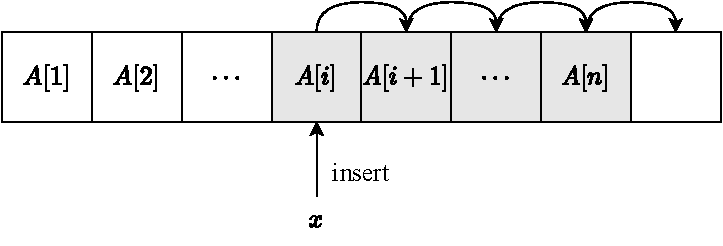
\includegraphics[scale=0.7]{img/array-shift.ps}
  \caption{将元素$x$插入数组$A$中的第$i$个位置}
  \label{fig:array-shift}
\end{figure}

从左向右扫描时,如果数组的长度为$n$,插入位置为$i$,我们需要扫描前面$i$个元素,然后进行$n-i+1$次移动,最后将$x$插入到第$i$个位置。也就是说,从左向右扫描会遍历整个数组。相反,如果从右向左扫描,我们最多只需要检查$i$个元素,并且一边扫描一边将元素向右移动。

下面的Python例子程序实现了上述算法。

\lstset{language=Python}
\begin{lstlisting}
def isort(xs):
    n = len(xs)
    for i in range(1, n):
        x = xs[i]
        j = i - 1
        while j >= 0 and x < xs[j]:
            xs[j+1] = xs[j]
            j = j - 1
        xs[j+1] = x
\end{lstlisting}

这一实现也存在一些变形,例如下面C语言的例子程序。它的操作次数比之前给出的方法要多一些。

\lstset{language=C}
\begin{lstlisting}
void isort(Key* xs, int n) {
    int i, j;
    for(i=1; i<n; ++i)
        for(j=i-1; j>=0 && xs[j+1] < xs[j]; --j)
            swap(xs, j, j+1);
}
\end{lstlisting}

这是因为交换函数\texttt{swap}通常需要一个中间变量,如下:

\begin{lstlisting}
void swap(Key* xs, int i, int j) {
    Key temp = xs[i];
    xs[i] = xs[j];
    xs[j] = temp;
}
\end{lstlisting}

若内循环的次数为$m$,上述C程序总共需要$3m$次赋值操作,而我们给出的算法及其Python实现使用shift来代替swap,它只需要$m+2$次赋值操作。

我们也可以提供单独的\textproc{Insert}()函数,然后在插入算法中调用它。我们略过这些细节,读者可以作为练习尝试这些不同的实现。

尽管有这些实现上的差异,从左向右也好,从右向左也好,所有这些插入算法的复杂度都是$O(n)$的,其中$n$为序列的长度。因此插入排序的总体复杂度为$O(n^2)$。

\begin{Exercise}

\begin{itemize}
\item 定义单独的插入函数,并在通用的插入排序算法中调用它。请尝试用命令式的方式和函数式的方式给出不同的实现。
\end{itemize}

\end{Exercise}

% ================================================================
% Improvement 1
% ================================================================

\section{改进一,二分查找}
\index{插入排序!二分查找}

人的大脑是如何快速在一手牌中找到插入位置的?答案明显不是逐一扫描。任何时刻,我们手中的牌都是已序的,因此我们可以用二分查找来搜索插入位置。

我们将在后面的章节中专门详细讨论搜索算法。本节仅仅对二分查找做一个简单介绍。

下面的排序算法改为调用二分查找来确定插入位置:

\begin{algorithmic}[1]
\Function{Sort}{$A$}
  \For{$i \gets 2$ to $|A|$}
    \State $x \gets A[i]$
    \State $p \gets $ \Call{Binary-Search}{$A[1...i-1], x$}
    \For{$j \gets i$ down to $p$}
      \State $A[j] \gets A[j-1]$
    \EndFor
    \State $A[p] \gets x$
  \EndFor
\EndFunction
\end{algorithmic}

我们不再逐一扫描元素,考虑数组中的片断$\{A[1], ..., A[i-1] \}$已经有序了。假设它们是单调增的,我们需要找到一个位置$j$使得$A[j-1] \leq x \leq A[j]$。我们可以先检查中间的元素$A[\lfloor i/2 \rfloor]$。如果$x$比它小,我们需要接下来递归地在前一半序列进行二分查找;否则我们需要查找后一半序列。

由于我们每次都排除掉一半元素,所以这一过程需要$O(\lg n)$的时间来找到插入位置。

\begin{algorithmic}[1]
\Function{Binary-Search}{$A, x$}
  \State $l \gets 1$
  \State $u \gets 1+|A|$
  \While{$l < u$}
    \State $m \gets \lfloor \frac{l+u}{2} \rfloor$
    \If{$A[m] = x$}
      \State \Return $m$ \Comment{找到一个重复元素}
    \ElsIf{$A[m] < x$}
      \State $l \gets m+1$
    \Else
      \State $u \gets m$
    \EndIf
  \EndWhile
  \State \Return $l$
\EndFunction
\end{algorithmic}

这一改进并不能提高插入排序的复杂度,结果仍然是$O(n^2)$。此前的算法进行了$O(n^2)$次比较和$O(n^2)$次移动,使用二分查找后,比较次数变成了$O(n \lg n)$,但是移动次数还是$O(n^2)$。

下面的Python例子程序实现了这一改进。

\lstset{language=Python}
\begin{lstlisting}
def isort(xs):
    n = len(xs)
    for i in range(1, n):
        x = xs[i]
        p = binary_search(xs[:i], x)
        for j in range(i, p, -1):
            xs[j] = xs[j-1]
        xs[p] = x

def binary_search(xs, x):
    l = 0
    u = len(xs)
    while l < u:
        m = (l+u)/2
        if xs[m] == x:
            return m
        elif xs[m] < x:
            l = m + 1
        else:
            u = m
    return l
\end{lstlisting}

\begin{Exercise}
使用递归来实现二分查找。编程语言不必限定为函数式的。
\end{Exercise}

% ================================================================
% Improvement 2
% ================================================================

\section{改进二,使用链表}
\index{插入排序!链表插入排序}

虽然我们通过二分查找,将搜索插入位置的时间降低为$O(n \lg n)$,但是移动元素的时间仍然是$O(n^2)$的。由于序列是使用数组存储的,我们无法避免这个耗时的操作。数组在内存中连续存储元素,插入操作必然需要通过连续的移动以空出位置。我们也可以尝试用链表来存储序列,这样插入操作就可以由线性时间$O(n)$提高到常数时间$O(1)$。

\be
  insert(A, x) = \left \{
  \begin{array}
  {r@{\quad:\quad}l}
  \{ x \} & A = \phi \\
  \{ x \} \cup A & x < a_1 \\
  \{ a_1 \} \cup insert(\{ a_2, a_3, ... a_n\}, x)& otherwise
  \end{array}
\right.
\ee

这一算法可以翻译为下面的Haskell例子程序。

\begin{lstlisting}[style=Haskell]
insert [] x = [x]
insert (y:ys) x = if x < y then x:y:ys else y:insert ys x
\end{lstlisting}

本章开头部份给出的插入排序定义,可以通过调用这一函数来完成。

\begin{lstlisting}[style=Haskell]
isort [] = []
isort (x:xs) = insert (isort xs) x
\end{lstlisting}

或者用fold来实现:

\begin{lstlisting}[style=Haskell]
isort = foldl insert []
\end{lstlisting}

我们也可以用命令式方式实现链表的插入排序。令函数\textproc{Key}($x$)返回节点$x$存储的元素,函数\textproc{Next}($x$)用以访问链表中的下一个节点。

\begin{algorithmic}[1]
\Function{Insert}{$L, x$}
  \State $p \gets$ NIL
  \State $H \gets L$
  \While{$L \neq$ NIL $\land $ \Call{Key}{$L$} $<$ \Call{Key}{$x$}}
    \State $p \gets L$
    \State $L \gets $ \Call{Next}{$L$}
  \EndWhile
  \State \Call{Next}{$x$} $\gets L$
  \If{$p =$ NIL}
    \State $H \gets x$
  \Else
    \State \Call{Next}{$p$} $\gets x$
  \EndIf
  \State \Return $H$
\EndFunction
\end{algorithmic}

下面的C语言例子代码定义了链表的节点:

\lstset{language=C}
\begin{lstlisting}
struct node {
    Key key;
    struct node* next;
};
\end{lstlisting}

根据此定义,插入程序可以实现如下:

\begin{lstlisting}
struct node* insert(struct node* lst, struct node* x) {
    struct node *p, *head;
    p = NULL;
    for(head = lst; lst && x->key > lst->key; lst = lst->next)
        p = lst;
    x->next = lst;
    if(!p)
        return x;
    p->next = x;
    return head;
}
\end{lstlisting}

我们也可以不用基于指针或者引用的数据结构,而通过另一个索引数组来实现链表。对于任何数组元素$A[i]$,$Next[i]$保存了$A[i]$下一个元素的索引。也就是说$A[Next[i]]$是$A[i]$的下一个元素。我们还需要一个变量来记录链表的表头。即索引$i_0$是的$A[i_0]$是链表中的第一个元素。我么可以使用$Next[\perp] = i_0$来代表这一特殊变量。

利用这种索引链表,插入算法可以定义如下:

\begin{algorithmic}[1]
\Function{Insert}{$A, Next, i$}
  \State $j \gets \perp$
  \While{$Next[j] \neq$ NIL $\land A[Next[j]] < A[i]$}
    \State $j \gets Next[j]$
  \EndWhile
  \State $Next[i] \gets Next[j]$
  \State $Next[j] \gets i$
\EndFunction
\end{algorithmic}

其中$\perp$表示索引表$Next$的头部。$Next[\perp]$给出了$A$中哪个元素是链表的表头。当实现这一算法时,我们可以在数组$A$的长度之上,再多给$Next$数组申请一个额外元素,并使用$Next$数组的最后一个元素来记录表头的索引。

下面的Python例子程序实现了索引链表的插入排序。

\lstset{language=Python}
\begin{lstlisting}
def isort(xs):
    n = len(xs)
    next = [-1]*(n+1)
    for i in range(n):
        insert(xs, next, i)
    return next

def insert(xs, next, i):
    j = -1
    while next[j] != -1 and xs[next[j]] < xs[i]:
        j = next[j]
    next[j], next[i] = i, next[j]
\end{lstlisting}

虽然使用链表后,插入操作降低为常数时间。但是我们必须遍历链表才能找到合适的插入位置。整个排序算法需要进行$O(n^2)$次比较。与数组不同,链表不支持随机访问(random access),我们不能利用二分查找在链表中搜索插入位置。

\begin{Exercise}
\begin{itemize}
\item 选择一种命令式编程语言,实现完整的链表插入排序算法。
\item 使用索引数组链表,排序结果是一个重新排列的索引。给出一个方法,根据新的索引,重新排列数组元素。
\end{itemize}
\end{Exercise}

% ================================================================
% Final improvement
% ================================================================

\section{使用二叉搜索树的最终改进}
\index{插入排序!二叉搜索树}

我们似乎钻进了死胡同:必须同时提高查找的速度和插入的速度,单独提高其中的一个仍然会保持$O(n^2)$的复杂度。

我们希望使用二分查找,这是唯一能把比较次数降低到$O(\lg n)$的方法。另一方面,我们必须改变数据结构,因为我们不能在普通数组中实现常数时间的插入。

这使我们想到了hello world数据结构―二叉搜索树。它本身就被定义为支持二分查找。同时,一旦找到了插入的位置,我们可以在常数$O(1)$时间插入一个新节点。

于是,我们最终获得了下面的算法:

\begin{algorithmic}[1]
\Function{Sort}{$A$}
  \State $T \gets \phi$
  \For{each $x \in A$}
    \State $T \gets $ \Call{Insert-Tree}{$T, x$}
  \EndFor
  \State \Return \Call{To-List}{$T$}
\EndFunction
\end{algorithmic}

其中函数\textproc{Insert-Tree}()和\textproc{To-List}()的定义在上一章。

根据我们对二叉搜索树的分析,树排序的性能为$O(n \lg n)$,达到了基于比较的排序算法的时间下限(\cite{Knuth-V3}第180-193页、\cite{CLRS}第167页)。

\section{小结}
本章展示了插入排序的进化过程。在经典的教科书中,插入排序通常作为第一个排序算法被介绍。它的思路简单直观,但是性能确是平方级别的。我们没有仅仅停留在这个结论上,而是设法分析它的性能瓶颈,并从不同方向上试图改进。我们首先尝试使用二分查找来减少比较操作,接着通过使用链表改变数据结构来改善插入操作。最后我们将两种改进结合起来,从而进化到了树排序。

\ifx\wholebook\relax \else
\begin{thebibliography}{99}

\bibitem{wiki-bubble-sort}
http://en.wikipedia.org/wiki/Bubble\_sort

\bibitem{CLRS}
Thomas H. Cormen, Charles E. Leiserson, Ronald L. Rivest and Clifford Stein.
``Introduction to Algorithms, Second Edition''. (《算法导论》中文版)ISBN:0262032937. The MIT Press. 2001

\bibitem{Knuth-V3}
Donald E. Knuth. ``The Art of Computer Programming, Volume 3: Sorting and Searching (2nd Edition)''. Addison-Wesley Professional; 2 edition (May 4, 1998) ISBN-10: 0201896850 ISBN-13: 978-0201896855

\end{thebibliography}

\end{document}
\fi
